\frame
{
\frametitle{Análisis Cualitativo de Riesgos}
\begin{itemize}
	\item Evalúa la \textbf{prioridad} de los riesgos identificados usando:
	\begin{itemize}
		\item Probabilidad de ocurrencia.
		\item El \textbf{impacto} correspondiente sobre los objetivos del
			proyecto si los riesgos efectivamente ocurren, tales como:
		\begin{itemize}
			\item Costos
			\item Cronograma
			\item Alcance
			\item Calidad
		\end{itemize}
	\end{itemize}
\end{itemize}
\begin{columns}
	\begin{column}{0.6\textwidth}
	\end{column}
	\begin{column}{0.4\textwidth}
		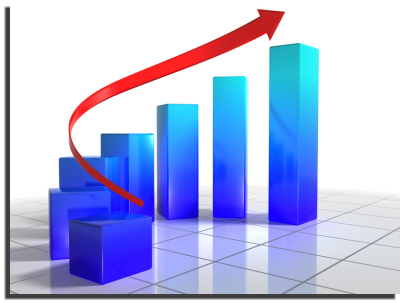
\includegraphics[width=3cm]{img/quality}
	\end{column}
\end{columns}
}

\frame
{
\frametitle{Análisis Cualitativo de Riesgos}
\begin{block}{Definición}
	El Análisis Cualitativo de Riesgos es normalmente una forma rápida de
	\textbf{establecer prioridades} para la Planificación de la Respuesta a los Riesgos.
\end{block}
}


\frame
{
\frametitle{Análisis Cualitativo de Riesgos}
\framesubtitle{Entradas}
\begin{columns}
	\begin{column}{0.8\textwidth}
		\begin{itemize}
			\item<1-> Registro de Riesgos.
			\item<2-> \textbf{Plan} de administración de Riesgos.
			\item<3-> Declaración del \textbf{alcance} del Proyecto.
			\item<4-> Activos organizacionales del Proceso.
		\end{itemize}
	\end{column}
	\begin{column}{0.2\textwidth}
		
\includegraphics[width=2cm]{img/input}
	\end{column}
\end{columns}
}

\frame
{
\frametitle{Análisis Cualitativo de Riesgos}
\framesubtitle{Herramientas y Técnicas}
\begin{columns}
	\begin{column}{0.8\textwidth}
		\begin{itemize}
			\item<1-> Probabilidad de riesgos y \textbf{evaluación} de impactos.
			\item<2-> \textbf{Matriz} de probabilidad e impacto.
			\item<3-> Evaluación de la calidad de los datos de los riesgos.
			\item<4-> \textbf{Categorización} de Riesgos.
			\item<5-> Evaluación de la \textbf{urgencia} de los riesgos.
			\item<6-> Juicio experto.
		\end{itemize}
	\end{column}
	\begin{column}{0.2\textwidth}
		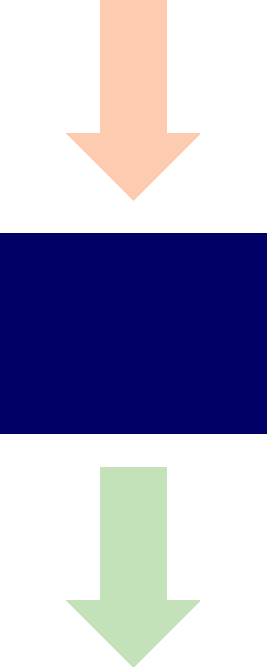
\includegraphics[width=2cm]{img/tools}
	\end{column}
\end{columns}
}

\frame
{
\frametitle{Análisis Cualitativo de Riesgos}
\framesubtitle{Salidas}
\begin{columns}
	\begin{column}{0.8\textwidth}
		Actualización de los registros de riesgos.
		\begin{itemize}
			\item<1-> Lista de prioridades de los riesgos del proyecto.
			\item<2-> Riesgos agrupados por \textbf{categorías}.
			\item<3-> Causas de riesgos o \textbf{áreas} que requieren una atención particular.
			\item<4-> Lista de riesgos que requieren respuesta \textbf{cercana} al equipo de trabajo.
			\item<5-> Lista de riesgos para un análisis y respuesta adicional.
			\item<6-> Lista de seguimiento de riesgos de baja prioridad.
			\item<7-> \textbf{Tendencias} en el resultado del análisis de riesgos cualitativo.
		\end{itemize}
	\end{column}
	\begin{column}{0.2\textwidth}
		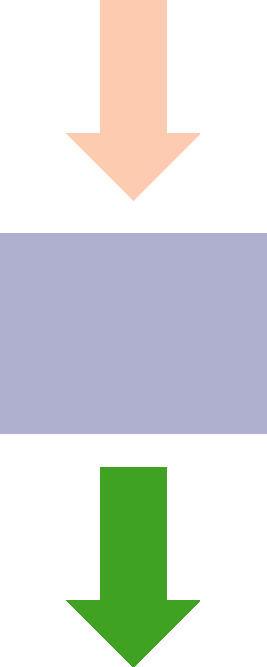
\includegraphics[width=2cm]{img/output}
	\end{column}
\end{columns}
}
